\subsection{Signatures of the quark-gluon plasma in small systems}
\label{sec:qgp_small}

The umbrella term ``small systems'' covers many different collision scenarios, each with its own advantages and challenges.
Generally, \pxp, \pxA, \AxAlight, and peripheral \AxA\ collisions can all be considered small systems.
Here, \AxAlight\ refers to light-ion collisions with mass number $A\lesssim 30$.
Light-ion data have only recently become available at RHIC (2026) and the LHC (2025).

Evidence for QGP formation includes partonic energy loss and collective flow.
As the system size decreases from that of central \AxA\ collisions, these experimental signatures are expected to weaken as the fireball, if formed, becomes progressively smaller.

\subsubsection{Collectivity in small systems}

Flow-like signatures have been observed in \pxp~\cite{HION-2015-09}, \pxPb~\cite{HION-2012-13}, \pxAu, \dxAu, and \HexAu~\cite{PHENIX:SmallFlow}, \OxO, \NexNe~\cite{HION-2025-02}, and peripheral \PbxPb~\cite{HION-2016-06}.
\TCR{Discuss the OSU model and add plots of flow observables.}
Collectivity has also been studied in systems even ``smaller'' than those listed above, such as electron--positron annihilation measured by the ALEPH detector at LEP~\cite{Belle:collective}.
The collectivity signal in $e^{+}e^{-}$ collisions was not significant and could be explained by \textsc{Pythia}6.

\subsubsection{\texorpdfstring{\pxp}{pp} collisions as a no jet quneching baseline}

Jet energy loss is not observed in \pxp\ collisions, as demonstrated by the success of pQCD calculations in describing \pxp\ data.
For example, measurements of the balance between an electroweak boson ($\gamma$ or $Z$) and a recoiling jet show that, on average, the boson and jet momenta agree with NLO predictions~\cite{STDM-2011-27}.
Since the electroweak boson does not interact strongly with the medium, any partonic energy loss would affect only the jet.
Therefore, jet quenching in \pxp\ collisions would produce a net momentum imbalance that would disagree with pQCD predictions.
Figure~\ref{fig:qgp_small_observables}(a) shows that the photon--jet momentum balance in \pxp\ collisions is consistent with pQCD predictions, while the corresponding \PbxPb\ data exhibit an imbalance~\cite{HION-2018-06}.
\begin{figure}[H]
    \centering
    \begin{subfigure}[t]{0.49\linewidth}
        \centering
        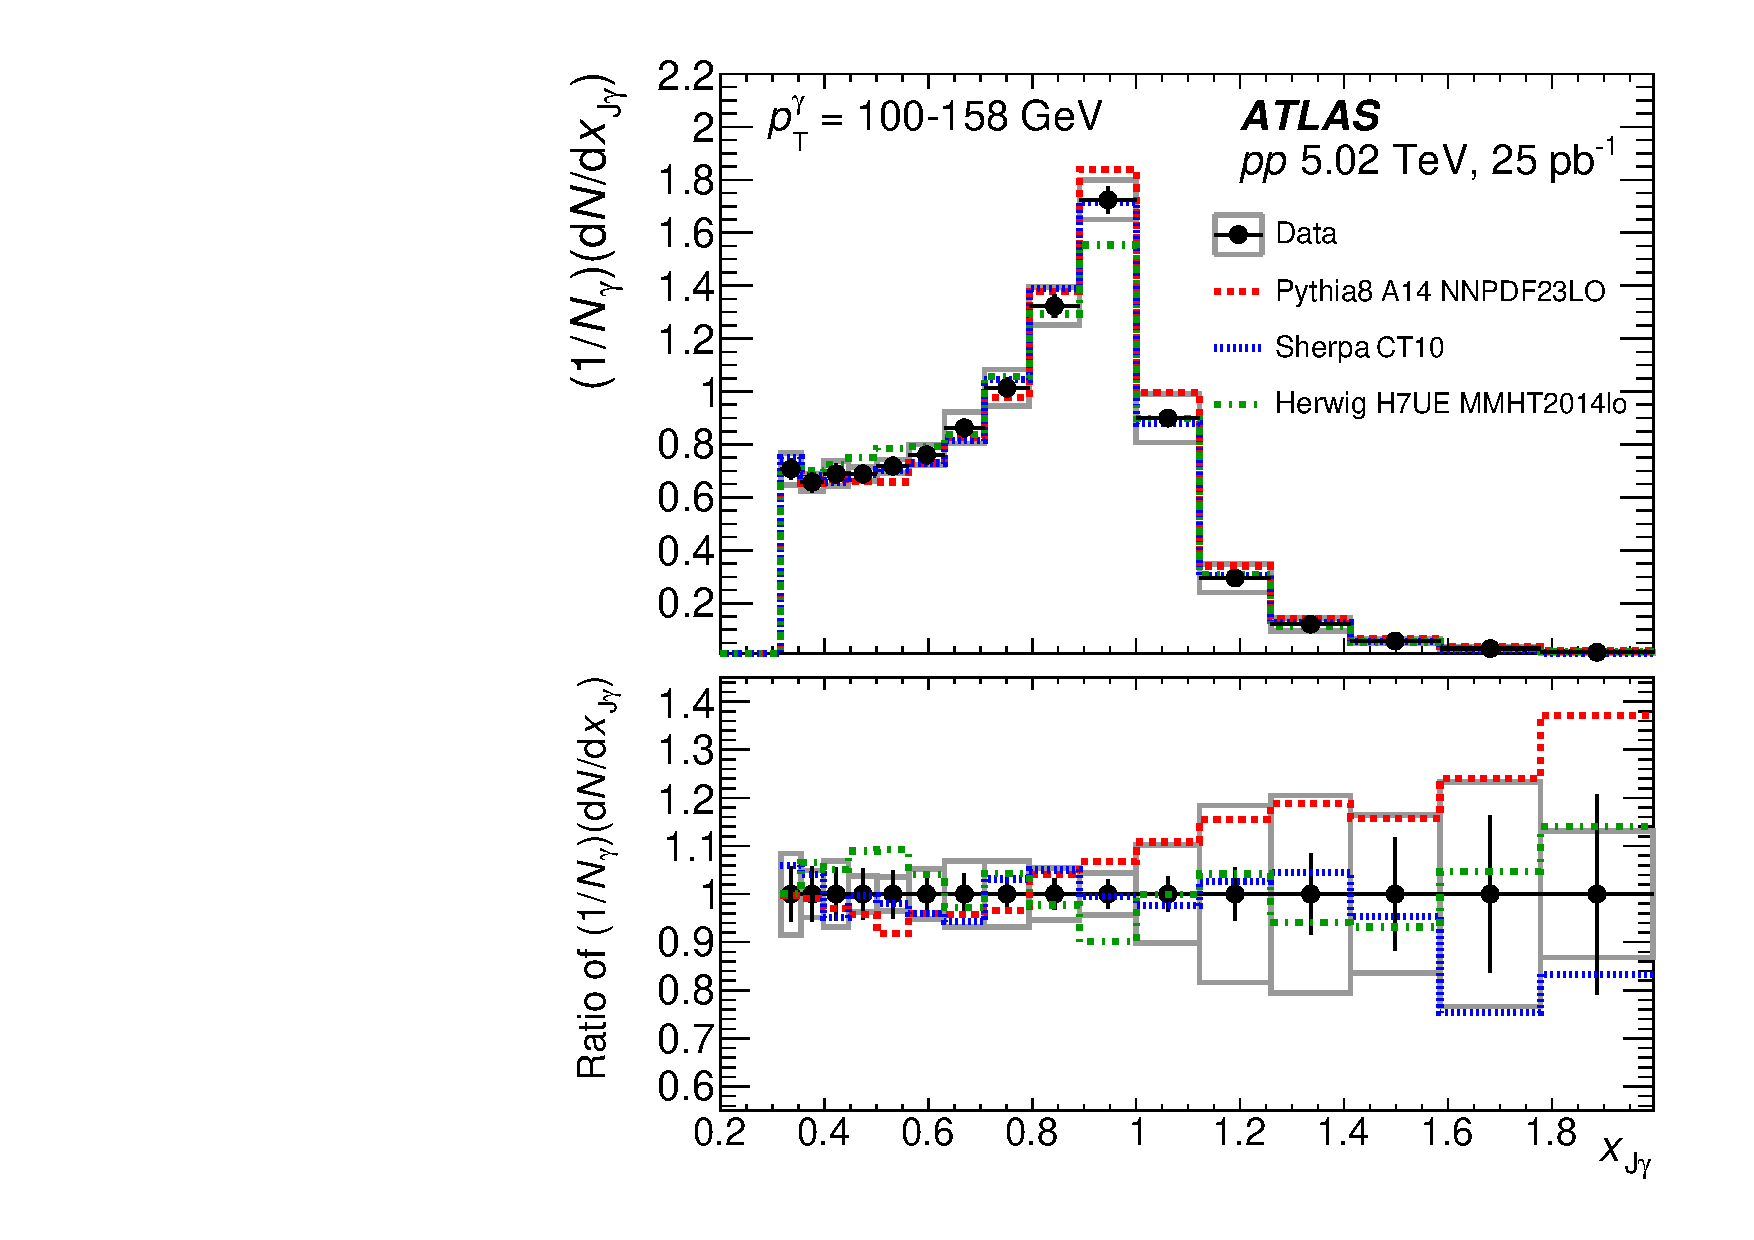
\includegraphics[
            width=\linewidth,
            alt={ATLAS photon--jet momentum balance in proton--proton and lead--lead collisions compared with pQCD predictions.}
        ]{chapters/background/sections/qgp_small/figures/HION201608-xjgamma.pdf}
    \end{subfigure}
    \hfill
    \begin{subfigure}[t]{0.49\linewidth}
        \centering
        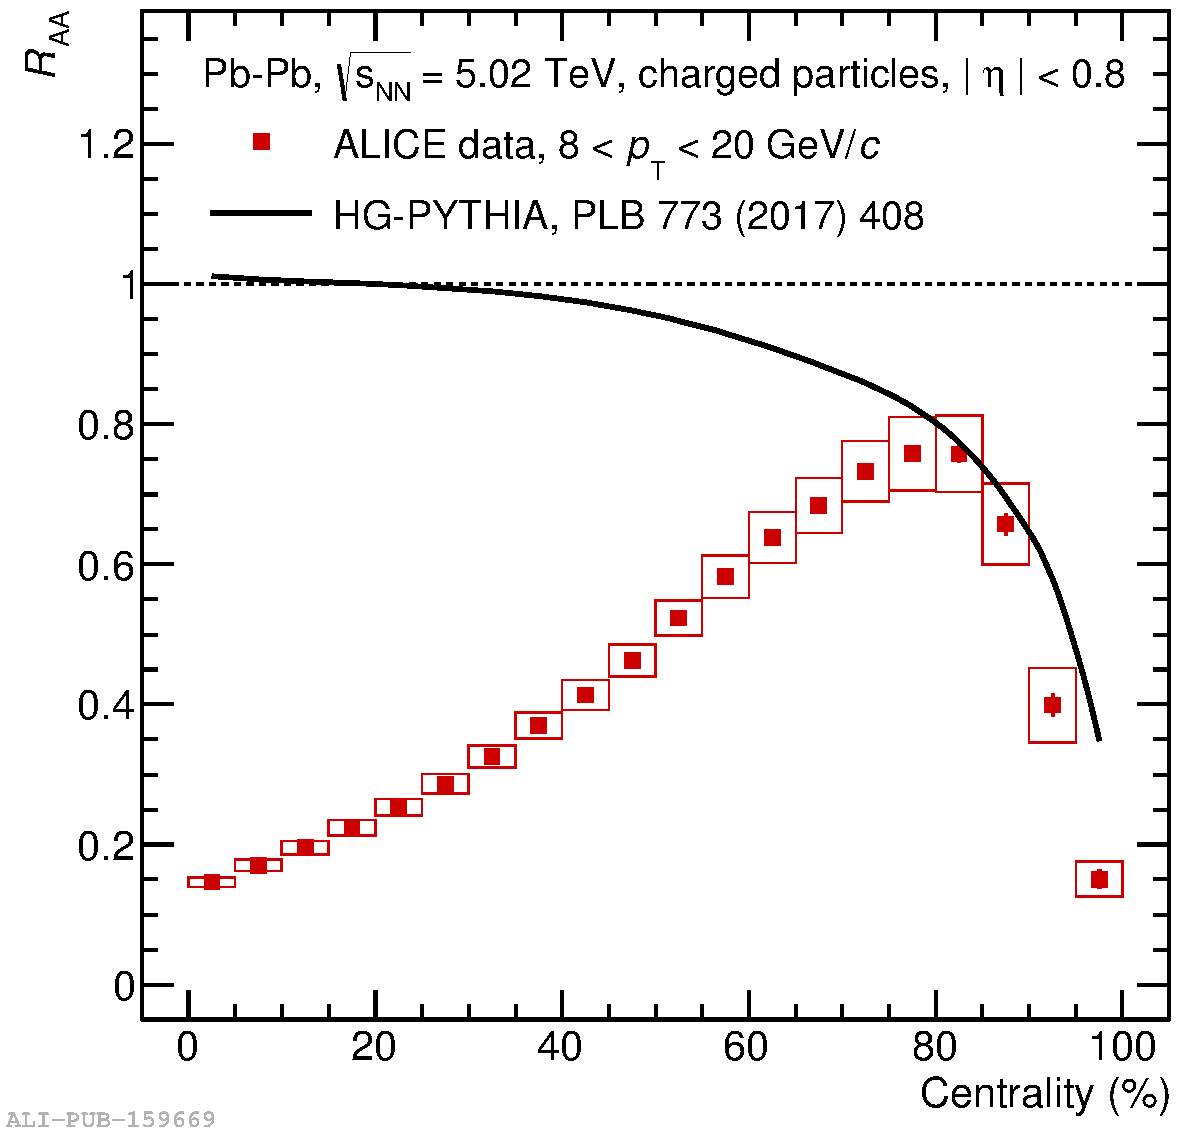
\includegraphics[
            width=\linewidth,
            alt={ALICE charged-hadron nuclear modification factor versus centrality, with a model describing peripheral suppression without jet quenching.}
        ]{chapters/background/sections/qgp_small/figures/2018-May-29-ppp_raa_fitconst.pdf}
    \end{subfigure}
    \caption{Measurements relevant to jet quenching in small and peripheral collision systems. In \pxp\ collisions, photon--jet momentum balance agrees with pQCD predictions, whereas the very peripheral charged-hadron suppression can be described by a model without jet quenching~\cite{HION-2018-06,ALICE:periphBias}.}
    \label{fig:qgp_small_observables}
\end{figure}

\subsubsection{CJet quenching in peripheral \texorpdfstring{\AxA}{AA} collisions}

Jet-quenching observables in peripheral \AxA\ collisions show suppression relative to \pxp\ collisions; however, interpreting this suppression is challenging.
Glauber modeling of peripheral collisions is associated with larger uncertainties because, at large impact parameters, the $N_{\mathrm{elem}}$ dependence is dominated by multiplicity fluctuations rather than geometry.
Additionally, events containing a hard process are correlated with higher soft underlying-event activity~\cite{CentBias:periphBias}.
This effect is small at large \NPART, where it is largely washed out, but its relative impact increases as \NPART\ decreases.
In the right panel of Figure~\ref{fig:atlas_hadron_jet_raa}, the jet \Raa\ is approximately $0.8$ at a \PT\ of 50 \GeV, but substantial uncertainties in \TAA\ (about 10\%) complicate its interpretation.
For very peripheral collisions (greater than 80\% centrality), the right panel of Figure~\ref{fig:qgp_small_observables} shows that the apparent suppression of charged-hadron \Raa\ in \PbxPb\ collisions can be described by a \pythia\ toy model with a HIJING Glauber initial state and no jet quenching~\cite{ALICE:periphBias,CentBias:periphBias}.
Beyond \Raa, correlation measurements (such as dijets and $\gamma$+jet pairs) have been shown to be more robust against centrality biases~\cite{CentBias:OO}.
Figure~\ref{fig:xj_absolute_yields} shows that the yield of balanced dijets is slightly suppressed relative to \pxp\ in the 60--80\% centrality interval, although the significance of this deviation has not been evaluated~\cite{HION-2018-28}.
The most peripheral \Jaa\ measurement reported is for the 40--60\% centrality interval, where the ratio is clearly different from unity~\cite{HION-2024-03}.
The effects of nPDFs and centrality biases on these measurements have not been rigorously evaluated, so definitive conclusions about the presence of jet quenching remain elusive.

\subsubsection{Jet quenching in \texorpdfstring{\pxA}{pA} collisions}

Measurements of inclusive-hadron and jet \Raa\ in \pxPb\ collisions at the LHC and \dxAu\ collisions at RHIC show no clear jet-quenching signal as seen in Figure~\ref{fig:qgp_small_pPb_Rp}.
The charged hadron \Raa\ is approximattly unity for hadrons with \PT\ > 5 \GeV, and is consistent with the two pQCD predictions provided.
The supression at very low \PT\ can be explained by nPDF effects.
The jet \Raa\ is at or above unity across measurments from ATLAS~\cite{HION-2013-08}, ALICE~\cite{ALICE:jetpPb}, CMS~\cite{CMS-HIN-14-001}, and PHENIX~\cite{PHENIX:jetpPb}.
\begin{figure}[H]
    \centering
    \begin{subfigure}[t]{0.49\linewidth}
        \centering
        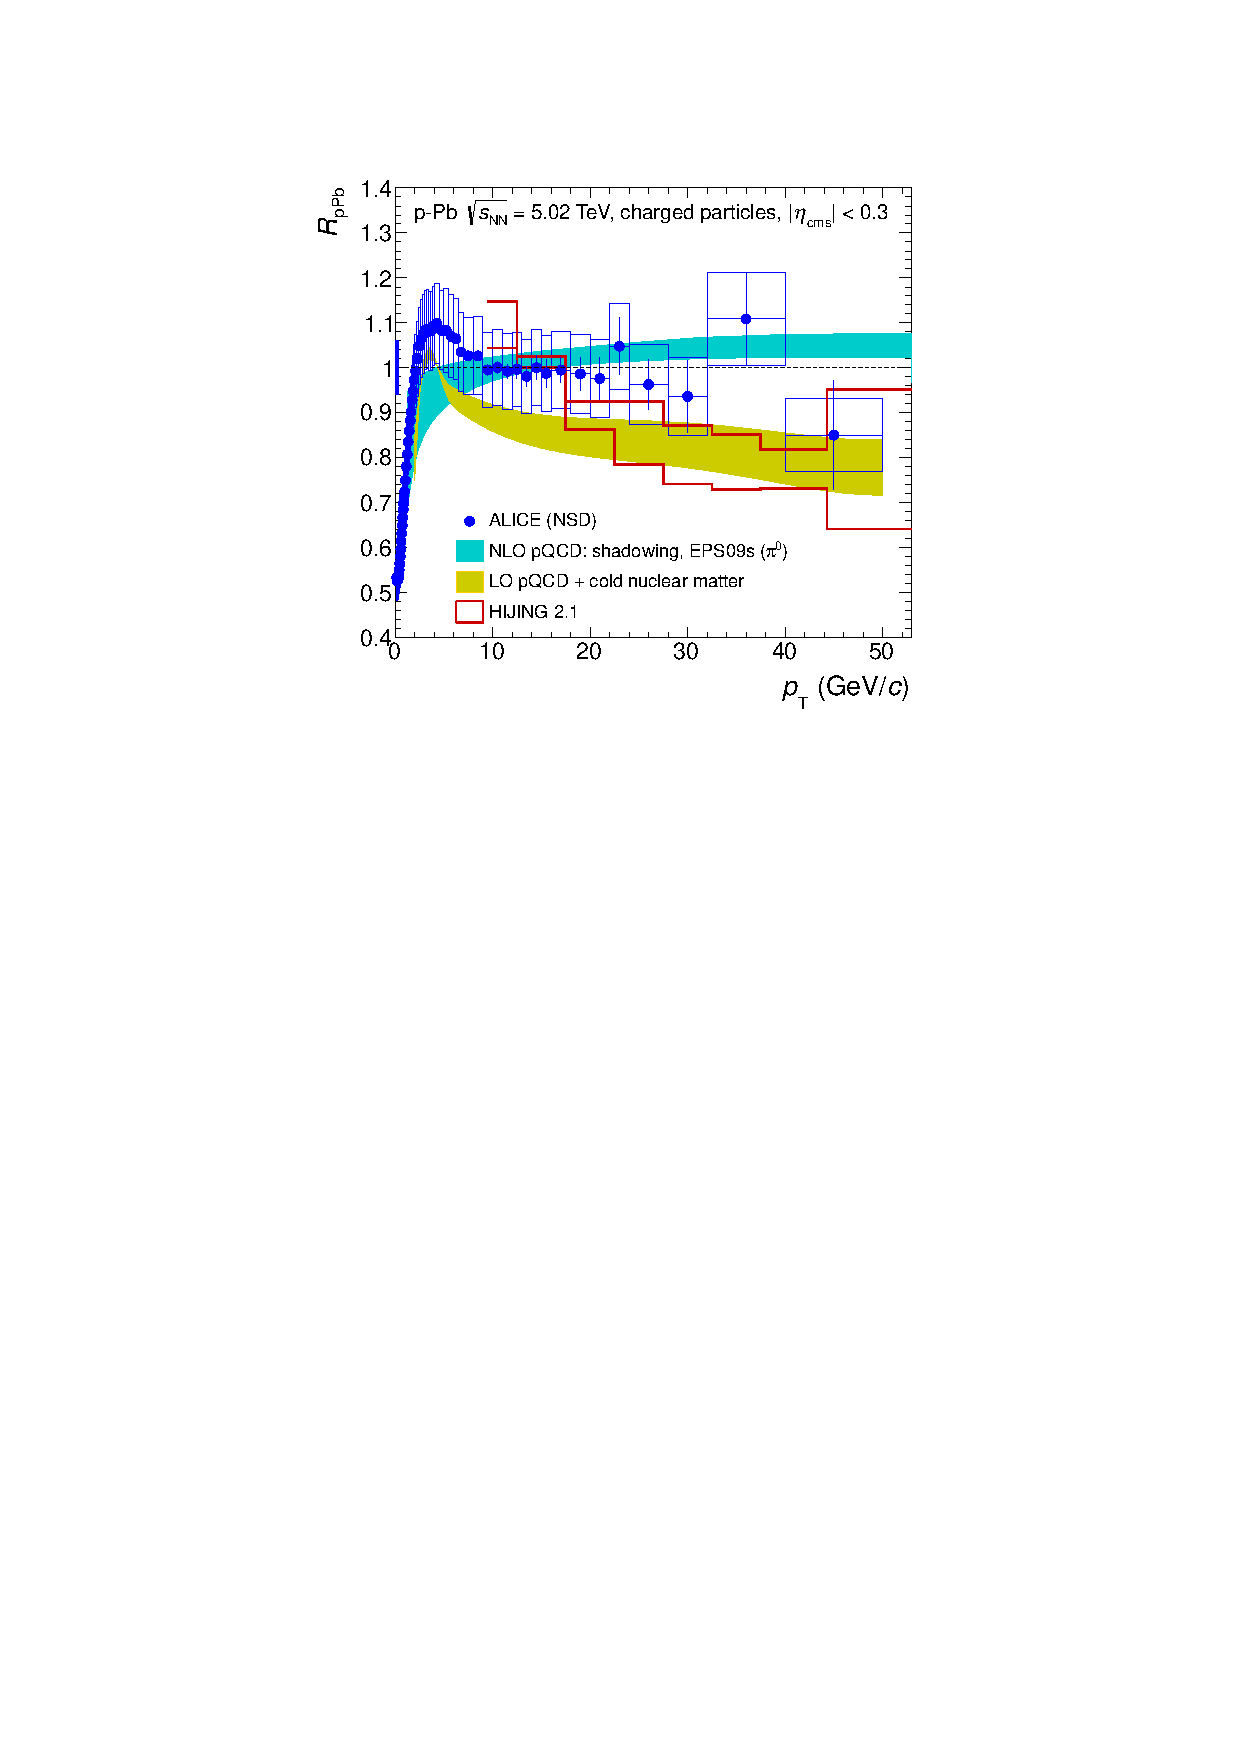
\includegraphics[
            width=\linewidth,
            alt={ALICE charged-hadron nuclear modification factor in proton--lead collisions compared with theoretical predictions.}
        ]{chapters/background/sections/qgp_small/figures/RpPbHadronTheory.pdf}
    \end{subfigure}
    \hfill
    \begin{subfigure}[t]{0.49\linewidth}
        \centering
        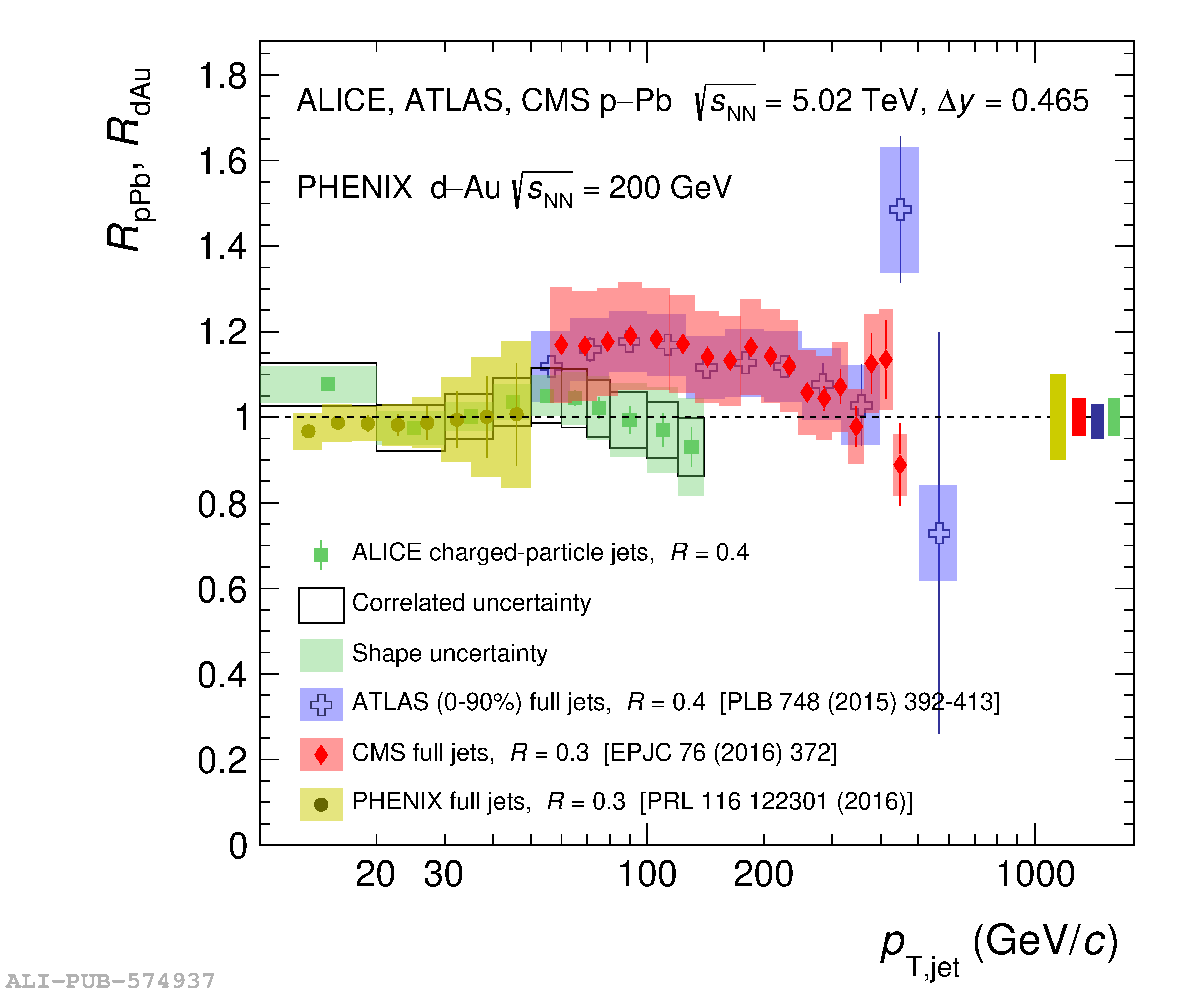
\includegraphics[
            width=\linewidth,
            alt={ALICE charged-particle jet nuclear modification factor in proton--lead collisions compared with reference data and theoretical predictions.}
        ]{chapters/background/sections/qgp_small/figures/RpPbComparison.pdf}
    \end{subfigure}
    \caption{ALICE measurements of the nuclear modification factor in \pxPb\ collisions. Left: charged-hadron $R_{\mathrm{pPb}}$ compared with theoretical predictions~\cite{ALICE:hadronpPb}. Right: charged-particle jet $R_{\mathrm{pPb}}$ compared with reference data and theoretical predictions~\cite{ALICE:jetpPb}. Other data from References~\cite{CMS-HIN-14-001,HION-2013-08,PHENIX:jetpPb}}
    \label{fig:qgp_small_pPb_Rp}
\end{figure}

Centrality-differential jet production has also been studied by PHENIX in \dxAu\ collisions and by ATLAS in \pxPb\ collisions~\cite{PHENIX:jetpPb,HION-2013-08}.
The centrality differentiated \Raa\ in \dxAu\ collisions is presented in the left panel of Figure~\ref{fig:qgp_small_centrality_jets}.
Focusing initally on the most central 0--20\% \dxAu\ class, the supressed \Raa\ is compatible with a small jet quneching signal and is compared with a model which includes medium induced radiation~\cite{pAEnergyLossModel}.
However, this model failed to describe the observed enhancement of the \Raa\ in peripheral collisions well above what could be expected from nPDF effects.
This findings for the \Raa\ were qualatiativly similar to the measurment by ATLAS~\cite{HION-2013-08}.
ATLAS defined the central to peripheral ratio of jet yeilds, \RCP, as
\begin{equation}
    \label{eq:RCP}
    R_{\mathrm{CP}} =
    \frac{\displaystyle
        \frac{1}{N_{\mathrm{evt}}\langle T_{p\mathrm{Pb}}\rangle}
        \frac{ \mathrm{d}^2N}
    {\mathrm{d}p_{\mathrm{T}}\,\mathrm{d}y} \bigg |_{\mathrm{central}}}
    {\frac{1}{N_{\mathrm{evt}}\langle T_{p+\mathrm{Pb}}\rangle}
        \frac{ \mathrm{d}^2N}
    {\mathrm{d}p_{\mathrm{T}}\,\mathrm{d}y} \bigg |_{\mathrm{peripheral}}}
\end{equation}

This represents the yield of central jet production to periphiral jet production, corrected for the difference in \NCOLL\ between the two classes.
The right panel of Figure~\ref{fig:qgp_small_centrality_jets} shows that the \RCP\ decreases as a function \textit{total jet energy} (\PT$\times \cosh\left(\langle y^* \rangle\right)$) where \YSTAR\ is the average rapidity of all jets in the event.
\begin{figure}[H]
    \centering
    \begin{subfigure}[t]{0.32\linewidth}
        \centering
        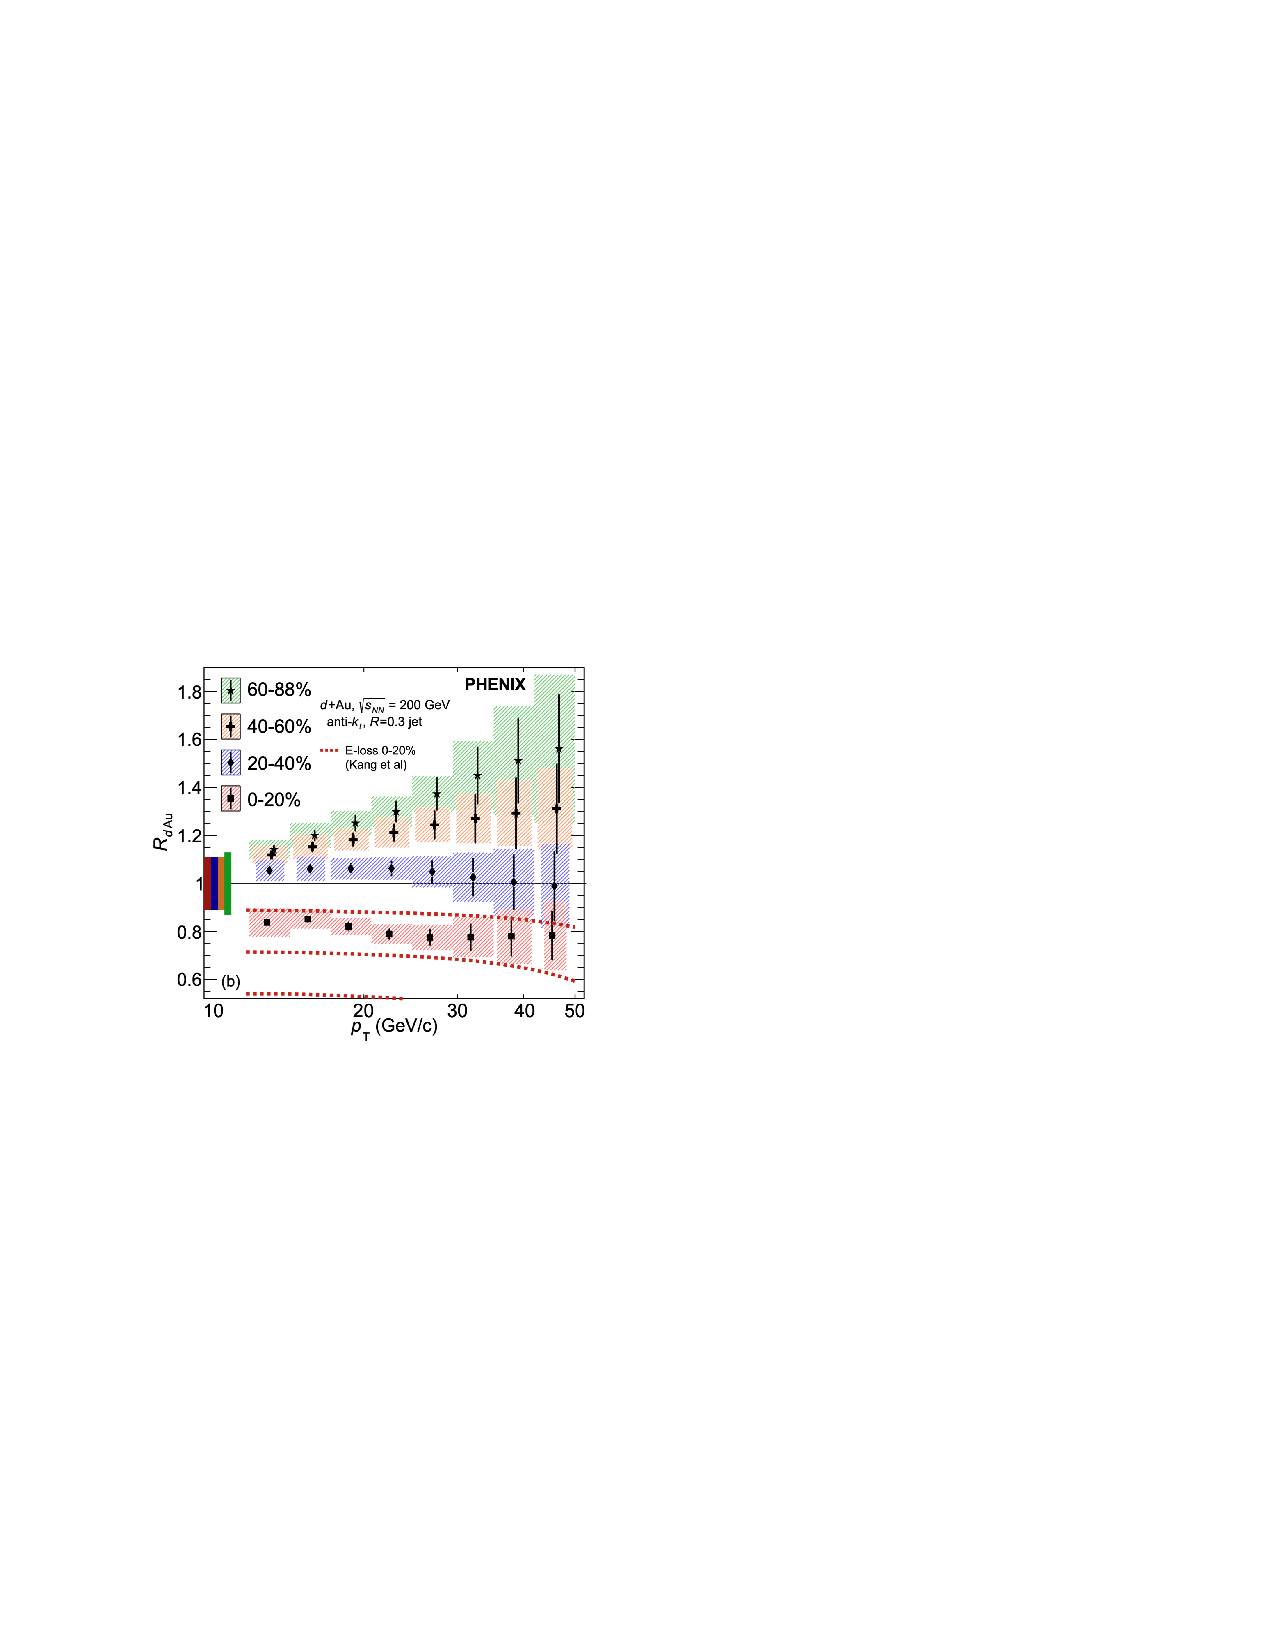
\includegraphics[
            width=\linewidth,
            alt={PHENIX nuclear modification factor for jets in deuteron--gold collisions shown in several centrality bins.}
        ]{chapters/background/sections/qgp_small/figures/PHENIXRdAu.pdf}
    \end{subfigure}
    \hfill
    \begin{subfigure}[t]{0.64\linewidth}
        \centering
        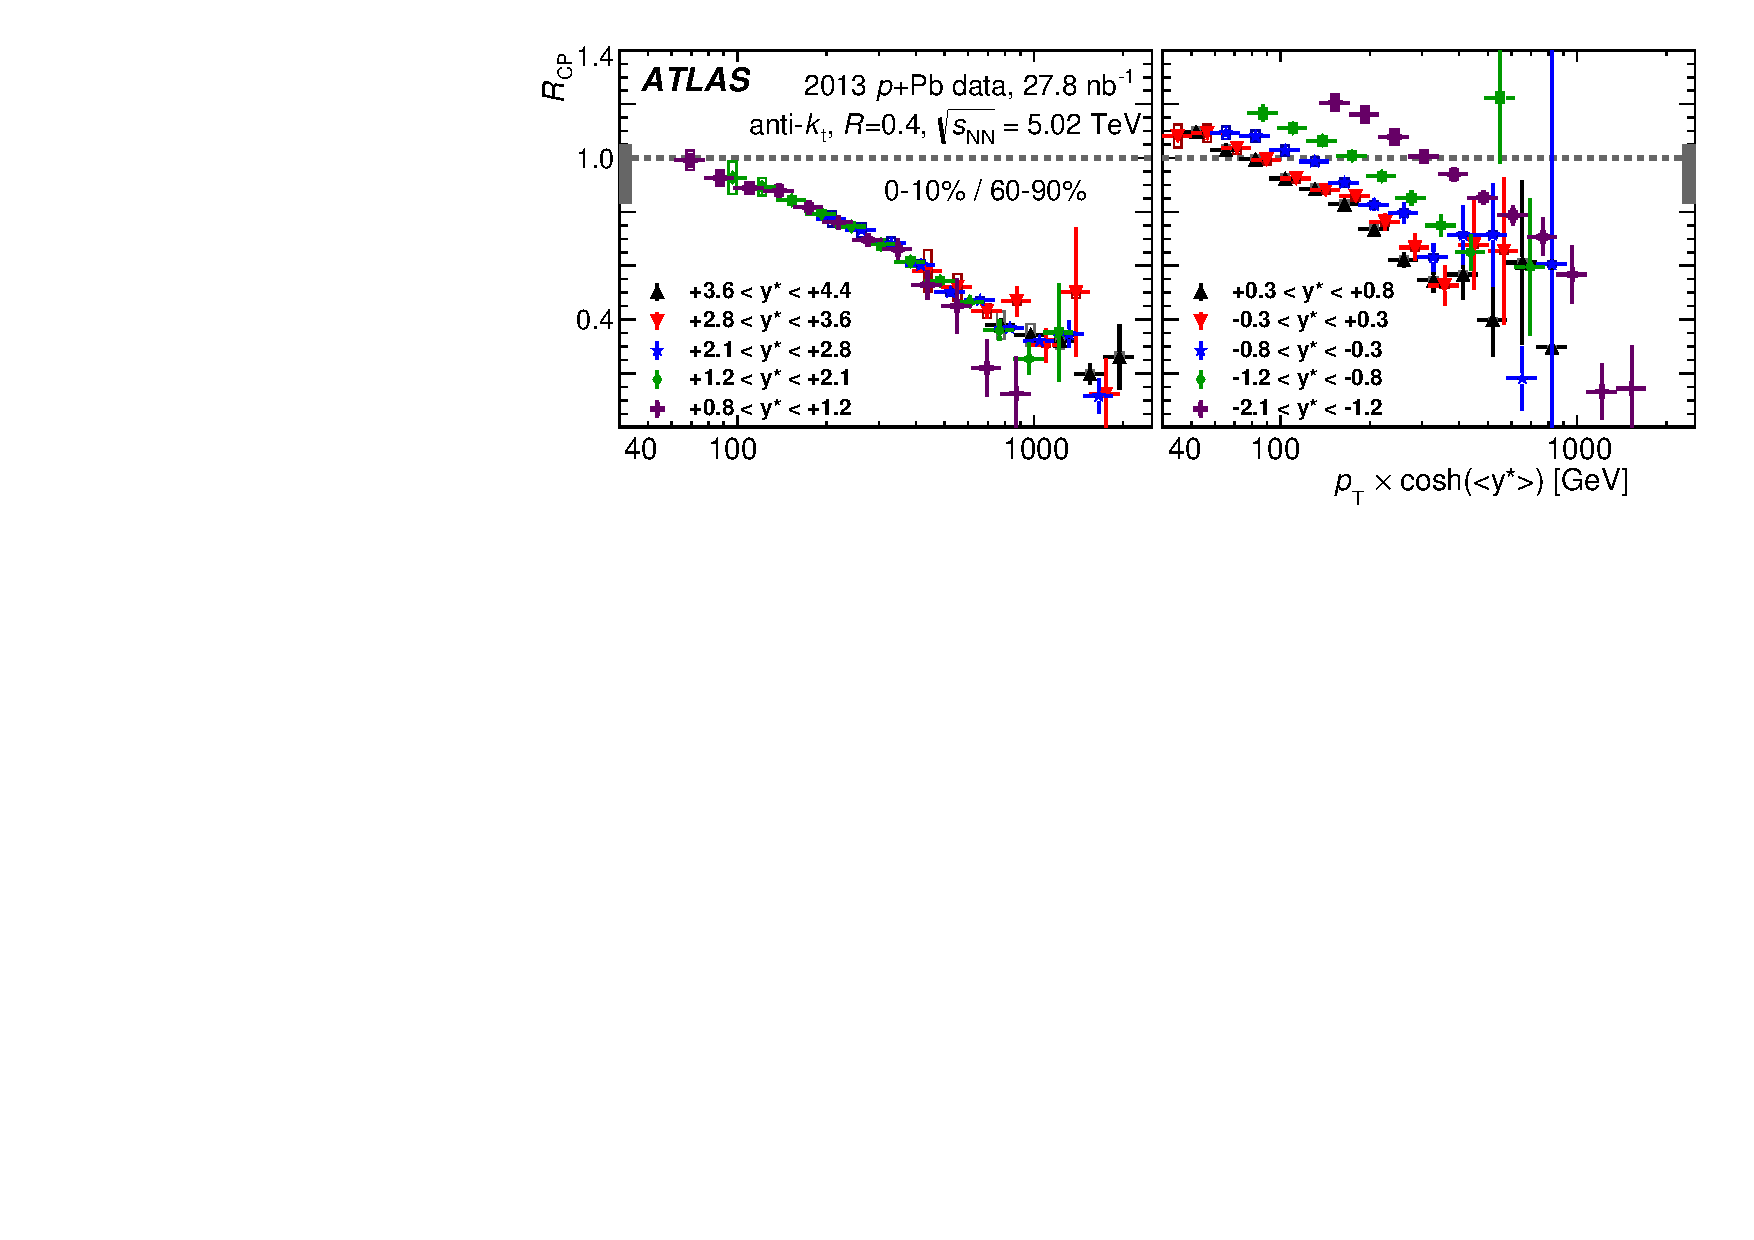
\includegraphics[
            width=\linewidth,
            alt={ATLAS central-to-peripheral ratio for jets in proton--lead collisions as a function of total jet energy at 5.02 TeV.}
        ]{chapters/background/sections/qgp_small/figures/ATLAS5p02Rcp.pdf}
    \end{subfigure}
    \caption{Centrality-dependent jet measurements in small collision systems. Left: PHENIX jet nuclear modification factor in d+Au collisions for several centrality intervals~\cite{PHENIX:jetpPb}. Right: ATLAS jet central-to-peripheral ratio, \RCP, as a function of total jet energy in \pxPb\ collisions at 5.02~TeV~\cite{HION-2013-08}.}
    \label{fig:qgp_small_centrality_jets}
\end{figure}

This suppression of \RCP\ as a function of jet $E$ was seen as a color transperency effect (see Section~\ref{sec:CT}) instead of evidence of jet energy loss.
Events with more jet $E$ are more likely to have been initialted by a high-$x$ parton in the proton, and thus be in a spatially compact tranvsertse configuration leading to fewer nucleon-nucleon collisions.
This centrality bias was discussed in Section~\ref{sec:pAcentBias} and it directly causes a migration to more periphiral centrralites, decreasing the \RCP.
This effect was studied in more detail by ATLAS through a triple differetial dijet yeild in 8.16 \TeV\ 

\TCR{Motivate the first measurement.}
\subsubsection{Jet quenching in peripheral \texorpdfstring{\AxAlight}{AAlight} collisions}

\TCR{Motivate the second measurement.}

{\color{red}
    \begin{itemize}
        \item Define small collision systems, such as proton--proton, proton--nucleus and light-ion collisions, and explain why QGP formation there was initially unexpected.
        \item Summarize collective signatures in small systems, including long-range correlations and flow-like patterns, and compare them with heavy-ion results.
        \item Discuss possible origins of these signatures, including hydrodynamic response, initial-state correlations, and the role of event activity.
        \item Review jet-quenching observables in pp and pPb collisions.
        \item Discuss how centrality-differential jet-quenching measurements in proton--nucleus collisions can be biased by projectile-configuration effects, as mentioned earlier, and motivate the first measurement in this thesis.
        \item Review jet-quenching observables in light-ion collisions.
        \item Motivate a measurement of dijet asymmetry in light-ion collisions as a method for searching for jet quenching.
    \end{itemize}
}
